\documentclass[conference]{IEEEtran}
\usepackage[utf8]{inputenc}
\usepackage[T5]{fontenc}
\usepackage{graphicx}
\usepackage{booktabs}
\usepackage{array}
\usepackage{tabularx}
\usepackage{url}
\usepackage{cite}
\usepackage{amsmath}

\graphicspath{{figures/}}

\begin{document}

\title{UniLake: So sánh kiến trúc Big Data truyền thống và Lakehouse hiện đại cho phân tích dữ liệu đa miền}

\author{
\IEEEauthorblockN{Giang Tuan Minh}
\IEEEauthorblockA{Information Systems\\
University of Engineering and Technology, VNU\\
Hanoi, Vietnam\\
giangtuanminh2703@gmail.com}
\and
\IEEEauthorblockN{Nguyen Van Bien}
\IEEEauthorblockA{Computer Science\\
University of Engineering and Technology, VNU\\
Hanoi, Vietnam\\
nguyenbien5102005@gmail.com}
\and
\IEEEauthorblockN{Le Van Tam}
\IEEEauthorblockA{Information Systems\\
University of Engineering and Technology, VNU\\
Hanoi, Vietnam\\
levantam12012005a@gmail.com}
\and
\IEEEauthorblockN{Nguyen Quang Hieu}
\IEEEauthorblockA{Computer Science\\
University of Engineering and Technology, VNU\\
Hanoi, Vietnam\\
nguyenquanghieu1032005@gmail.com}
\and
\IEEEauthorblockN{Dinh Van An}
\IEEEauthorblockA{Information Systems\\
University of Engineering and Technology, VNU\\
Hanoi, Vietnam\\
andinh3072005@gmail.com}
}

\maketitle

\begin{abstract}
Báo cáo này trình bày UniLake, một nguyên mẫu lakehouse cục bộ nhằm so sánh đường xử lý file-based Parquet fallback với đường xử lý bảng Apache Iceberg trên MinIO, đồng thời đặt kết quả đó trong bối cảnh so sánh giữa kiến trúc Big Data truyền thống và kiến trúc lakehouse hiện đại. Kiến trúc tham chiếu truyền thống gồm Kafka, Spark, HDFS/Parquet và Presto/Trino; kiến trúc hiện đại gồm Redpanda, Spark, MinIO, Apache Iceberg và Spark SQL. Thực nghiệm sử dụng ba miền dữ liệu: giao dịch bán lẻ, dữ liệu văn bản sentiment và dữ liệu cảm biến IoT. Benchmark cục bộ chạy 3 lần cho mỗi bảng và mỗi đường lưu trữ, đo thời gian ghi, đọc/đếm và truy vấn tổng hợp. Kết quả cho thấy trong môi trường Docker cục bộ, đường Iceberg trên MinIO có thời gian trung bình thấp hơn Parquet fallback trong các thao tác được đo. Tuy nhiên, báo cáo không khái quát hóa Iceberg là luôn nhanh hơn Parquet, vì Iceberg là table format quản lý metadata/snapshot trên các file dữ liệu, còn Parquet là file format cột. Đóng góp chính của UniLake là một quy trình thực nghiệm có thể tái lập, phân biệt rõ bằng chứng benchmark cục bộ, bằng chứng học thuật/công khai và lập luận kiến trúc.
\end{abstract}

\begin{IEEEkeywords}
UniLake, Big Data, Lakehouse, Apache Spark, Apache Iceberg, Apache Parquet, MinIO, benchmark cục bộ.
\end{IEEEkeywords}

\section{Giới thiệu}

Trong nhiều hệ thống phân tích dữ liệu hiện đại, dữ liệu không còn xuất hiện dưới một định dạng duy nhất. Một pipeline phân tích thực tế thường phải kết hợp dữ liệu giao dịch có cấu trúc, văn bản ngắn đã gán nhãn, log sự kiện và tín hiệu cảm biến theo thời gian. Điều này làm cho bài toán Big Data không chỉ là bài toán lưu trữ khối lượng lớn, mà còn là bài toán tổ chức dữ liệu đa miền sao cho có thể xử lý, truy vấn, kiểm chứng và mở rộng bằng nhiều engine khác nhau.

Kiến trúc Big Data truyền thống thường được mô tả bằng chuỗi Kafka--Spark--HDFS/Parquet--Presto/Trino--Analytics. Trong kiến trúc này, Kafka đảm nhiệm ingestion dữ liệu luồng, Spark xử lý batch/SQL, HDFS lưu trữ dữ liệu phân tán, Parquet tối ưu lưu trữ cột, còn Presto/Trino cung cấp lớp truy vấn SQL tương tác. Mô hình này có lịch sử triển khai lâu dài và được hỗ trợ bởi nhiều công trình nền tảng. Tuy nhiên, khi áp dụng vào môi trường học tập hoặc prototype trên máy cá nhân, việc dựng đầy đủ HDFS, broker, query engine và catalog thường phát sinh chi phí vận hành đáng kể.

Kiến trúc lakehouse hiện đại tìm cách giảm khoảng cách giữa data lake và data warehouse bằng cách lưu dữ liệu trên object storage ở định dạng mở, đồng thời thêm lớp quản lý bảng, metadata, schema, snapshot và transaction log. Trong UniLake, đường hiện đại được hiện thực hóa bằng Redpanda, Spark, MinIO và Apache Iceberg. Đường thực nghiệm được so sánh trực tiếp là Spark ghi/đọc Parquet fallback theo thư mục và Spark ghi/đọc Iceberg table trên MinIO.

Mục tiêu của báo cáo là xây dựng một đánh giá thận trọng theo ba tầng bằng chứng. Tầng thứ nhất là benchmark cục bộ dựa trên các file CSV thật trong phạm vi đề tài. Tầng thứ hai là tài liệu học thuật và tài liệu chính thức về Kafka, HDFS, Spark, Presto, Lakehouse, Delta Lake, Iceberg và Parquet. Tầng thứ ba là lập luận kiến trúc nhằm giải thích vì sao table format có thể hữu ích ngay cả khi dữ liệu vật lý vẫn được lưu dưới dạng Parquet.

Tên hệ thống trong báo cáo là \textit{UniLake}. Báo cáo không mô tả UniLake như một hệ thống production-scale, mà như một nguyên mẫu Docker-first cho Windows/WSL2, có thể chạy lại, kiểm tra kết quả và phục vụ một báo cáo IEEE-style bằng tiếng Việt.

\section{Định nghĩa bài toán}

Bài toán trung tâm của UniLake là đánh giá một cách có kiểm soát sự khác biệt giữa hai đường lưu trữ/phân tích trên cùng một Spark engine:

\begin{itemize}
\item \textbf{Đường A -- Parquet fallback}: Spark làm sạch dữ liệu, ghi dữ liệu ra các thư mục Parquet, sau đó đọc lại và chạy truy vấn tổng hợp bằng Spark SQL.
\item \textbf{Đường B -- Iceberg trên MinIO}: Spark làm sạch cùng dữ liệu, ghi dữ liệu thành Iceberg table trong warehouse đặt trên MinIO, sau đó đọc lại bảng và chạy truy vấn tổng hợp tương đương.
\end{itemize}

Hai đường này không phải là so sánh ``Parquet thay thế Iceberg'' hoặc ``Iceberg thay thế Parquet''. Parquet là file format cột; Iceberg là table format quản lý metadata, snapshot, schema và danh sách data files. Trong nhiều cấu hình, Iceberg vẫn sử dụng Parquet làm định dạng file vật lý. Vì vậy, câu hỏi nghiên cứu hợp lệ hơn là: khi cùng dùng Spark và cùng một bộ dữ liệu, việc đặt một lớp table format Iceberg trên object storage cục bộ tạo ra workflow và kết quả benchmark như thế nào so với đọc/ghi Parquet trực tiếp theo thư mục?

Báo cáo cần trả lời bốn câu hỏi:

\begin{enumerate}
\item Prototype UniLake chứng minh được điều gì trong phạm vi cục bộ?
\item Các công trình học thuật và tài liệu chính thức nói gì về legacy Big Data stack và lakehouse/open table formats?
\item Những nhận định nào từ nguồn công khai được kết quả local hỗ trợ?
\item Những nhận định nào vẫn chưa được kiểm chứng do giới hạn phần cứng, dữ liệu và phạm vi triển khai?
\end{enumerate}

Để tránh kết luận sai, mọi phát biểu về hiệu năng trong báo cáo đều dựa trên \texttt{benchmark/results/benchmark\_results.csv}, \texttt{benchmark/results/benchmark\_summary.csv} hoặc các hình được sinh từ các file này. Nếu một thành phần không được triển khai trong core benchmark, báo cáo ghi rõ là chưa kiểm chứng.

\section{Công trình liên quan}

\subsection{Framework truyền thống}

Kafka được giới thiệu như một hệ thống messaging phân tán cho log processing, hướng tới việc thu thập và phân phối sự kiện ở thông lượng cao với độ trễ thấp~\cite{kafkaPaper}. Đóng góp của Kafka nằm ở mô hình distributed commit log, cho phép nhiều consumer xử lý cùng một luồng sự kiện theo nhu cầu online hoặc offline. Trong kiến trúc legacy của UniLake, Kafka đại diện cho lớp ingestion. Trong prototype, Redpanda được dùng như một lựa chọn nhẹ hơn và tương thích Kafka API, phù hợp hơn với môi trường Docker cục bộ.

HDFS là một nền tảng lưu trữ phân tán cho file lớn, tối ưu cho throughput và khả năng chịu lỗi trên cụm nhiều node~\cite{hdfsPaper}. HDFS đại diện cho thế hệ data lake on-premise, nơi dữ liệu thường được lưu thành file lớn và đọc bởi các engine xử lý phân tán. Tuy nhiên, HDFS không tự cung cấp các chức năng table management hiện đại như snapshot, schema evolution hoặc transaction log ở cấp bảng. Đây là một trong các động lực dẫn đến sự xuất hiện của lakehouse và open table formats.

Spark phát triển từ abstraction Resilient Distributed Dataset, sau đó trở thành một engine thống nhất cho batch, SQL, streaming và machine learning~\cite{rddPaper,sparkCacm}. Trong UniLake, Spark là điểm chung của cả hai đường thực nghiệm, giúp benchmark tập trung vào lớp storage/table format thay vì so sánh hai engine xử lý khác nhau. Điều này cũng làm giảm nhiễu phương pháp luận: cùng phiên bản Spark, cùng logic làm sạch dữ liệu, cùng truy vấn tổng hợp và cùng số lần chạy.

Presto được mô tả như một engine ``SQL on Everything'', cho phép truy vấn phân tán trên nhiều nguồn dữ liệu khác nhau~\cite{prestoPaper}. Trong kiến trúc legacy, Presto hoặc Trino thường đứng ở lớp interactive SQL phía trên HDFS/Parquet hoặc object storage. UniLake chưa triển khai Trino/StarRocks trong benchmark lõi; do đó các engine này chỉ được dùng trong phần so sánh kiến trúc và future work.

\subsection{Parquet, Lakehouse và table formats}

Dremel là một hệ thống phân tích ad-hoc quy mô web, kết hợp cây thực thi nhiều cấp và biểu diễn dữ liệu cột cho nested records~\cite{dremelPaper}. Dù Dremel không phải Parquet, các ý tưởng về columnar representation và phân tích trên dữ liệu lớn là nền tảng quan trọng cho các định dạng cột trong hệ sinh thái Big Data. Parquet kế thừa định hướng tối ưu cho workload phân tích: đọc một tập cột con, nén hiệu quả và hỗ trợ predicate/filter pushdown ở mức engine.

Công trình Lakehouse của Armbrust và cộng sự lập luận rằng data lake và data warehouse có thể được hợp nhất bằng một kiến trúc mở, trong đó dữ liệu được lưu trên định dạng trực tiếp như Parquet/ORC và được quản lý bởi lớp metadata/table management~\cite{lakehousePaper}. Đây là khung lý thuyết chính của UniLake: hệ thống không cố thay thế Parquet, mà đặt Parquet trong một workflow có catalog và metadata rõ hơn.

Delta Lake là một ví dụ tiêu biểu về ACID table storage trên cloud object stores, dùng transaction log để cung cấp ACID, time travel và tối ưu thao tác metadata trên dữ liệu lớn~\cite{deltaLakePaper}. Dù UniLake chọn Iceberg thay vì Delta Lake, công trình Delta Lake vẫn có giá trị vì chỉ ra các vấn đề của data lake thuần file trên object store: thao tác metadata đắt, cập nhật nhiều object không nguyên tử và khó đảm bảo nhất quán trong workload phức tạp.

Apache Iceberg định nghĩa một table format quản lý các tập file dữ liệu lớn trên distributed file system hoặc object store. Đặc tả Iceberg mô tả bảng thông qua metadata files, schema, partition specs, snapshots, manifest lists và manifest files~\cite{icebergSpec}. Tài liệu Spark của Iceberg cũng khuyến nghị workflow ghi bằng DataFrameWriterV2, chẳng hạn \texttt{df.writeTo(t).create()} cho thao tác CTAS tương ứng~\cite{icebergSparkWrites}. Đây là API được dùng trong benchmark UniLake.

\subsection{Về so sánh Iceberg và Parquet fallback}

Trong quá trình khảo sát, nhóm không tìm thấy một bài báo học thuật chuẩn mực nào so sánh trực tiếp ``Iceberg với Parquet fallback'' như hai hệ thống cùng cấp. Điều này phù hợp về mặt khái niệm: Iceberg là table format còn Parquet là file format. Các bài báo liên quan chủ yếu so sánh kiến trúc lakehouse, transaction log/table format, hoặc phân tích giới hạn của data lake thuần file. Vì vậy, benchmark UniLake được viết là so sánh hai \textit{đường triển khai}: Spark + Parquet fallback và Spark + Iceberg table trên MinIO. Cách gọi này tránh nhầm lẫn rằng Iceberg và Parquet là hai định dạng file thay thế nhau.

\begin{table*}[htbp]
\centering
\caption{Tóm tắt công trình liên quan và liên hệ với UniLake}
\label{tab:related-work}
\begin{tabularx}{\textwidth}{p{0.16\textwidth}X X X}
\toprule
Công trình & Đóng góp chính & Giới hạn khi áp dụng trực tiếp & Liên hệ với UniLake \\
\midrule
Kafka~\cite{kafkaPaper} & Distributed log cho ingestion thông lượng cao. & Không giải quyết quản lý bảng phân tích. & Baseline ingestion; Redpanda là biến thể nhẹ hơn cho local. \\
HDFS~\cite{hdfsPaper} & Lưu trữ phân tán cho file lớn và throughput cao. & Triển khai local nặng; thiếu table metadata hiện đại. & Đại diện legacy storage. \\
Spark~\cite{rddPaper,sparkCacm} & Engine thống nhất cho batch, SQL, streaming và ML. & Spark local không đại diện cluster nhiều node. & Engine chung cho cả hai đường benchmark. \\
Presto~\cite{prestoPaper} & SQL phân tán trên nhiều nguồn dữ liệu. & Chưa chạy trong benchmark lõi. & Query layer mở rộng cho legacy/lakehouse. \\
Lakehouse~\cite{lakehousePaper} & Hợp nhất data lake và warehouse bằng định dạng mở và metadata. & Cần table format cụ thể để triển khai. & Khung lý thuyết của UniLake. \\
Delta Lake~\cite{deltaLakePaper} & ACID table storage trên object store. & Không phải table format được chọn trong prototype. & Bằng chứng về nhu cầu vượt qua data lake thuần file. \\
Iceberg~\cite{icebergSpec,icebergSparkWrites} & Metadata, snapshot, schema/partition evolution cho bảng phân tích. & Cần cấu hình catalog, S3A và runtime tương thích. & Table format chính của đường modern. \\
\bottomrule
\end{tabularx}
\end{table*}

\section{Nền tảng công nghệ}

\subsection{Parquet fallback}

Trong UniLake, Parquet fallback là đường lưu trữ trực tiếp theo thư mục: Spark ghi DataFrame đã chuẩn hóa thành file Parquet, sau đó đọc lại bằng Spark SQL. Tài liệu Spark 3.5.1 nêu rõ Spark SQL hỗ trợ đọc và ghi Parquet, đồng thời bảo toàn schema của dữ liệu gốc trong nhiều workflow DataFrame/SQL~\cite{sparkParquetDocs}. Parquet phù hợp với workload phân tích vì tổ chức dữ liệu theo cột, giúp engine chỉ đọc các cột cần thiết thay vì scan toàn bộ record theo hàng.

Tuy nhiên, Parquet tự thân không phải một hệ quản trị bảng. Khi dữ liệu được lưu thành nhiều file theo thư mục, các vấn đề như snapshot nhất quán, thay đổi schema, partition evolution, xóa/cập nhật logic, hoặc nhiều engine cùng đọc/ghi cần thêm lớp metadata bên ngoài. Vì vậy, Parquet fallback trong báo cáo được xem là baseline kỹ thuật, không phải đại diện đầy đủ cho toàn bộ legacy production stack.

\subsection{Apache Iceberg}

Iceberg là table format cho analytic datasets. Theo đặc tả Iceberg, trạng thái bảng được duy trì trong metadata files; mỗi thay đổi tạo metadata mới và snapshot biểu diễn trạng thái nhất quán của bảng tại một thời điểm~\cite{icebergSpec}. Iceberg không phủ nhận vai trò của Parquet; ngược lại, Iceberg có thể quản lý các data files ở định dạng Parquet, Avro hoặc ORC. Điểm khác biệt nằm ở lớp metadata, snapshot và quy tắc tiến hóa schema/partition.

Trong UniLake, Spark ghi Iceberg table bằng DataFrameWriterV2. Việc dùng API này phù hợp với khuyến nghị của Iceberg Spark docs vì hành vi ghi bảng rõ ràng hơn so với DataFrameWriterV1, hỗ trợ các thao tác create, replace, append và overwrite theo ngữ nghĩa bảng~\cite{icebergSparkWrites}.

\subsection{MinIO và object storage}

MinIO được dùng như object storage cục bộ tương thích S3~\cite{minioS3Compatibility}. Mục tiêu không phải mô phỏng đầy đủ cloud object storage ở quy mô production, mà tạo một endpoint S3A đủ nhẹ để Spark và Iceberg có thể ghi warehouse Iceberg. Cách triển khai này phù hợp với nguyên tắc Docker-first của đề tài: người dùng Windows chạy qua WSL2 Ubuntu, không cần cài native Spark, Hadoop, Java hoặc \texttt{winutils.exe}.

\subsection{Trino và StarRocks}

Trino và StarRocks không nằm trong core benchmark của UniLake. Tuy nhiên, chúng là các engine SQL tương tác quan trọng trong kiến trúc lakehouse. Tài liệu Trino và StarRocks đều mô tả khả năng truy cập Iceberg thông qua connector/catalog~\cite{trinoIcebergDocs,starrocksIcebergDocs}. Vì chưa được triển khai trong benchmark, mọi nhận định về Trino/StarRocks trong báo cáo chỉ được xem là định hướng mở rộng, không phải kết quả thực nghiệm.

\section{Phương pháp nghiên cứu}

Phương pháp của UniLake dựa trên nguyên tắc tam giác hóa bằng chứng: kết quả benchmark cục bộ, nguồn học thuật/tài liệu chính thức và lập luận kiến trúc. Cách tiếp cận này giúp tránh hai cực đoan: chỉ mô tả lý thuyết mà không có kết quả chạy được, hoặc chỉ nhìn số đo local rồi suy diễn quá mức sang production.

\subsection{Thiết kế benchmark}

Benchmark sử dụng cùng Spark engine cho cả hai đường lưu trữ. Với mỗi bảng, workflow gồm bốn bước:

\begin{enumerate}
\item Đọc dữ liệu đầu vào đã chuẩn hóa từ \texttt{data/benchmark\_input}.
\item Làm sạch và ép kiểu dữ liệu bằng Spark.
\item Ghi dữ liệu vào Parquet fallback hoặc Iceberg table.
\item Đọc lại để đếm số dòng và chạy truy vấn tổng hợp tương đương.
\end{enumerate}

Các chỉ số được đo gồm \texttt{write\_seconds}, \texttt{read\_seconds}, \texttt{query\_seconds}, \texttt{row\_count}, \texttt{run\_id}, \texttt{storage\_path}, \texttt{status} và \texttt{notes}. Mỗi tổ hợp bảng--đường lưu trữ được chạy 3 lần. Thời gian được đo bằng \texttt{time.perf\_counter()} trong script Python.

\subsection{Dữ liệu}

Dữ liệu được chuẩn hóa từ các CSV thật trong thư mục \texttt{data/raw}: Online Retail, Twitter Entity Sentiment training/validation và IoT telemetry. Script \texttt{src/prepare\_real\_csv\_data.py} tạo ba bảng benchmark-ready:

\begin{itemize}
\item \texttt{retail\_transactions}: giao dịch bán lẻ, có doanh thu dòng \texttt{revenue = quantity * unit\_price}.
\item \texttt{twitter\_sentiment}: tweet, entity, sentiment và độ dài văn bản.
\item \texttt{iot\_sensor\_events}: timestamp, device, nhiệt độ, độ ẩm, chỉ số khí và motion.
\end{itemize}

Sau bước lọc hợp lệ trong Spark benchmark, số dòng được đo là 531.283 dòng retail, 75.682 dòng sentiment và 405.184 dòng IoT. Đây là dữ liệu đủ lớn để có thời gian đo rõ ràng trong local, nhưng vẫn nhỏ hơn rất nhiều so với Big Data production.

\subsection{Nguyên tắc diễn giải}

Mọi kết quả hiệu năng chỉ được diễn giải trong phạm vi môi trường Docker cục bộ. Báo cáo không dùng benchmark này để tuyên bố rằng Iceberg luôn nhanh hơn Parquet hoặc modern stack luôn thay thế legacy stack. Nếu một nhận định đến từ tài liệu công khai nhưng không được prototype kiểm chứng, báo cáo đánh dấu là chưa kiểm chứng.

\section{Kiến trúc đề xuất}

\subsection{Kiến trúc legacy tham chiếu}

Hình~\ref{fig:legacy-architecture} mô tả baseline legacy: Kafka tiếp nhận sự kiện, Spark xử lý dữ liệu, HDFS/Parquet lưu trữ file, Presto/Trino cung cấp SQL analytics. Mô hình này phù hợp với nhiều hệ thống Big Data truyền thống vì các thành phần đã trưởng thành và có cộng đồng lớn. Tuy nhiên, khi triển khai đầy đủ trong local, stack này đòi hỏi nhiều service, nhiều cấu hình và tài nguyên tương đối cao.

\begin{figure}[htbp]
\centering
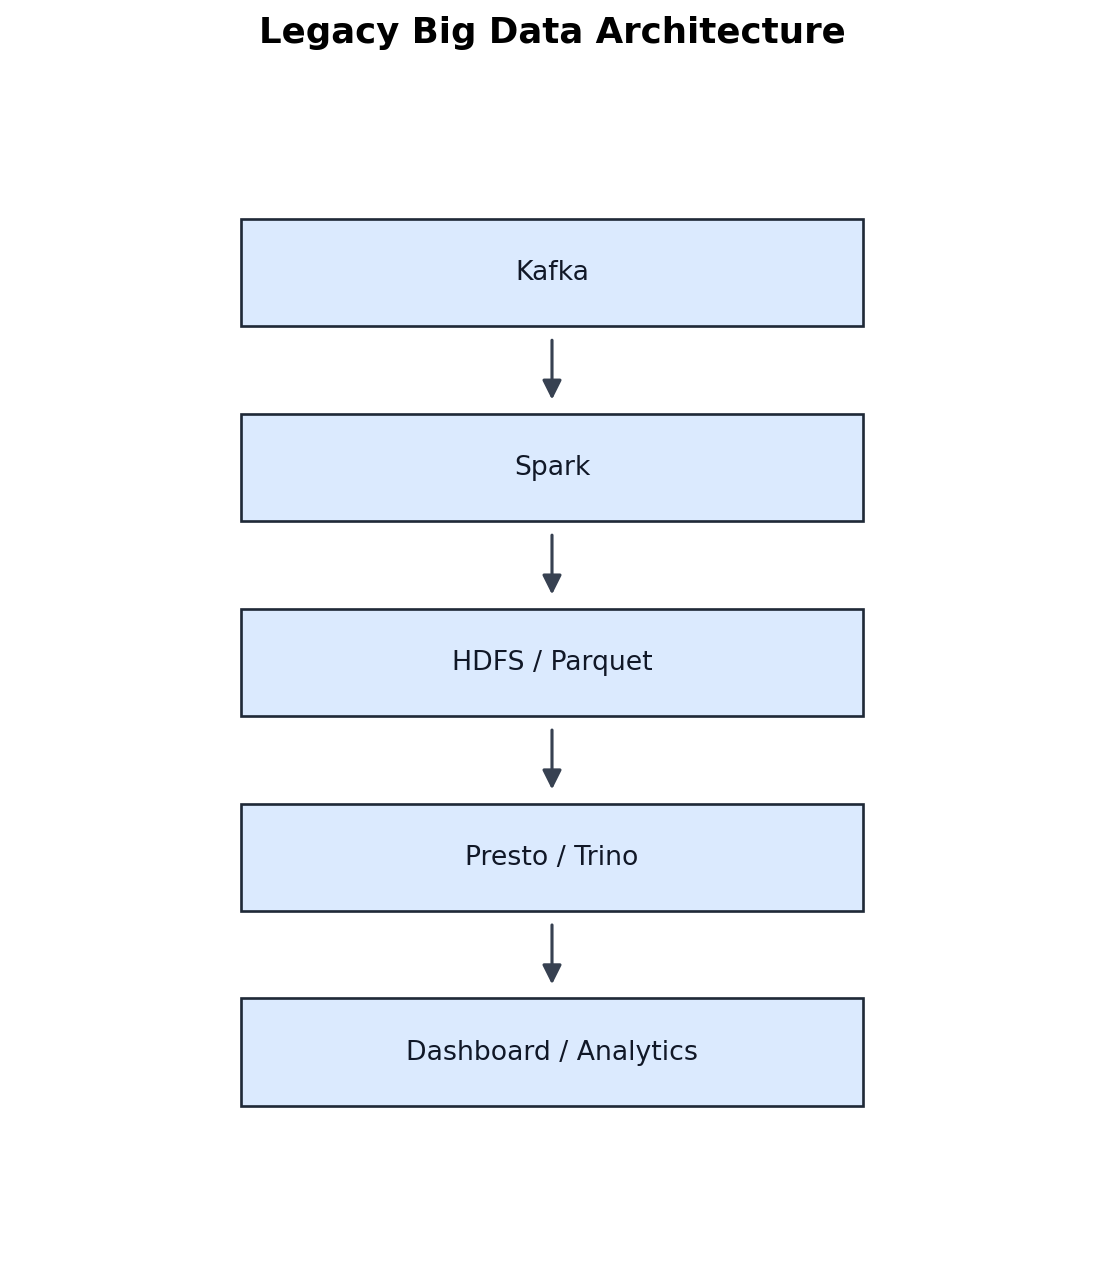
\includegraphics[width=0.48\textwidth]{architecture_legacy.png}
\caption{Kiến trúc Big Data truyền thống tham chiếu.}
\label{fig:legacy-architecture}
\end{figure}

\subsection{Kiến trúc modern của UniLake}

Hình~\ref{fig:modern-architecture} mô tả kiến trúc modern: Redpanda thay cho Kafka trong prototype nhẹ, Spark là engine xử lý, MinIO là object storage cục bộ, Iceberg là table format, Spark SQL là query layer chính. Trino/StarRocks được xem là phần mở rộng có thể thêm vào sau, nhưng không chặn benchmark lõi.

\begin{figure}[htbp]
\centering
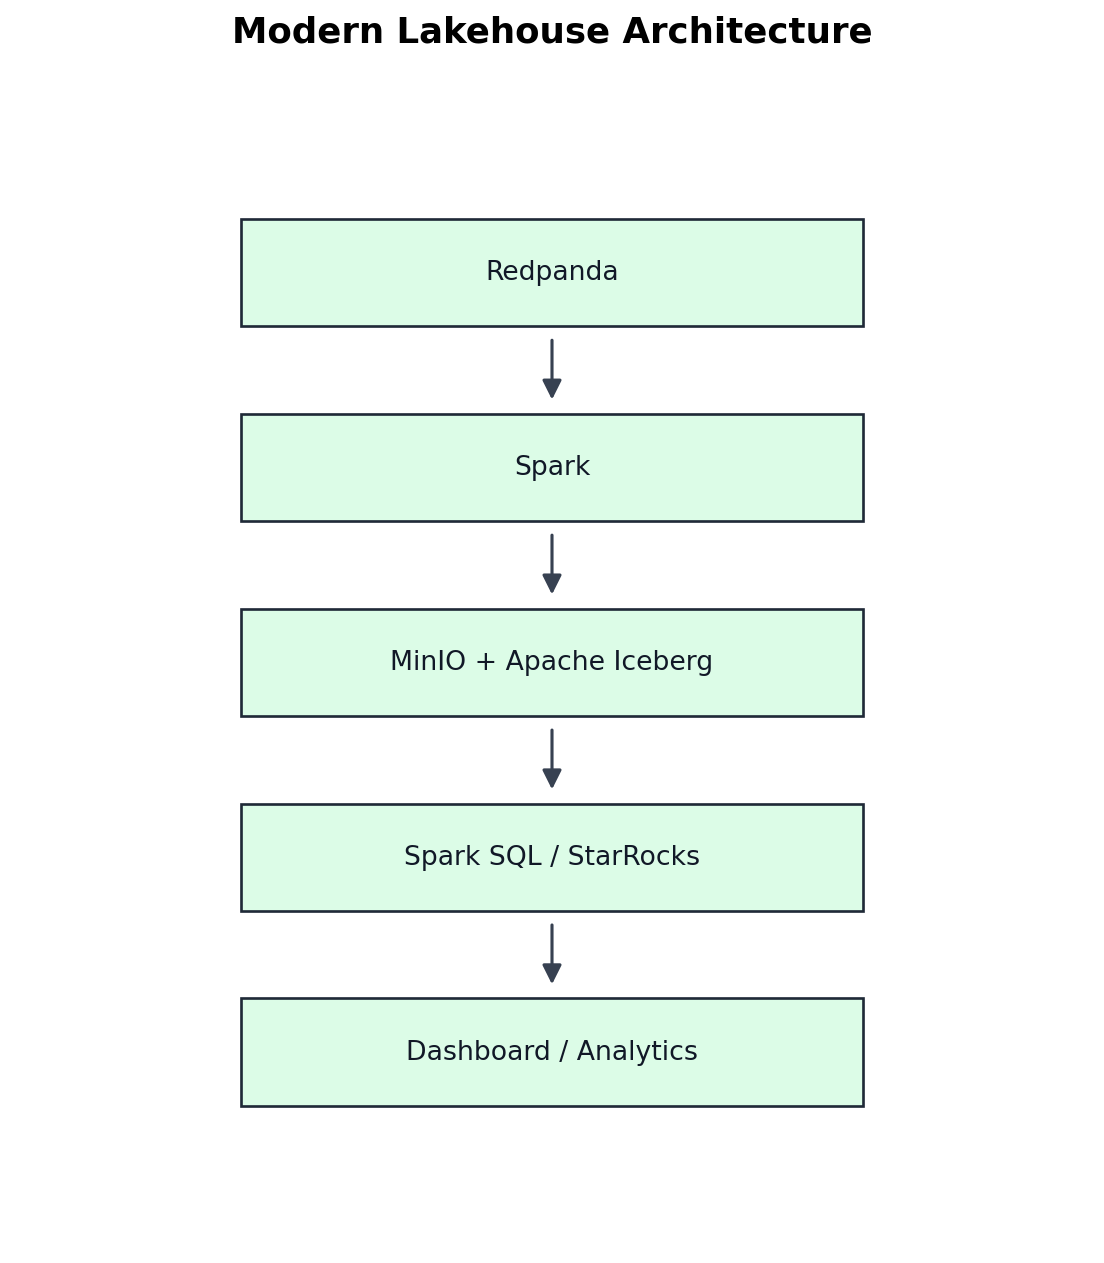
\includegraphics[width=0.48\textwidth]{architecture_modern.png}
\caption{Kiến trúc lakehouse hiện đại của UniLake.}
\label{fig:modern-architecture}
\end{figure}

Điểm cốt lõi của kiến trúc modern không phải là thay Parquet bằng Iceberg, mà là bổ sung lớp quản lý bảng trên object storage. Iceberg tạo ra abstraction bảng logic, trong khi dữ liệu vật lý vẫn có thể là file Parquet. Điều này làm cho hệ thống dễ mở rộng sang các engine khác hơn so với việc mỗi engine tự hiểu các thư mục Parquet rời rạc.

\begin{table}[htbp]
\centering
\caption{So sánh kiến trúc legacy và modern trong phạm vi UniLake}
\label{tab:architecture-comparison}
\begin{tabular}{p{0.25\linewidth}p{0.31\linewidth}p{0.31\linewidth}}
\toprule
Tiêu chí & Legacy Big Data & Modern Lakehouse \\
\midrule
Ingestion & Kafka & Redpanda tương thích Kafka API \\
Xử lý & Spark batch/SQL & Spark batch/SQL \\
Lưu trữ & HDFS hoặc Parquet thư mục & MinIO object storage \\
Định dạng dữ liệu & Parquet file & Iceberg table quản lý Parquet files \\
Metadata & Phụ thuộc catalog/engine & Metadata, snapshot, manifest của Iceberg \\
Query layer & Presto/Trino & Spark SQL, mở rộng Trino/StarRocks \\
\bottomrule
\end{tabular}
\end{table}

\section{Thiết lập thực nghiệm và kết quả}

\subsection{Môi trường chạy}

Benchmark được chạy bằng Docker Compose trong môi trường cục bộ. Spark container dùng Spark 3.5.1; Iceberg runtime dùng \texttt{org.apache.iceberg:iceberg-spark-runtime-3.5\_2.12:1.5.2}; Hadoop AWS dùng \texttt{hadoop-aws:3.3.4}; MinIO cung cấp endpoint S3A \texttt{http://minio:9000}. Kết quả được ghi vào \texttt{benchmark/results/benchmark\_results.csv} và tổng hợp vào \texttt{benchmark/results/benchmark\_summary.csv}.

\subsection{Workload truy vấn}

Ba truy vấn tổng hợp được dùng để đại diện cho ba miền dữ liệu:

\begin{itemize}
\item Retail: top quốc gia theo doanh thu, số hóa đơn và tổng doanh thu.
\item Sentiment: số tweet theo nhãn sentiment.
\item IoT: tổng hợp theo thiết bị và giờ, gồm số sự kiện, nhiệt độ trung bình, độ ẩm trung bình và số lần motion.
\end{itemize}

\subsection{Kết quả benchmark}

Bảng~\ref{tab:benchmark-summary} trình bày thời gian trung bình của 3 lần chạy cho mỗi bảng và mỗi đường lưu trữ. Tất cả 18 dòng raw benchmark đều có \texttt{status=OK}. Các số liệu trong bảng được lấy trực tiếp từ \texttt{benchmark/results/benchmark\_summary.csv}.

\begin{table*}[htbp]
\centering
\caption{Kết quả benchmark Parquet fallback và Iceberg trên MinIO}
\label{tab:benchmark-summary}
\begin{tabular}{llrrrr}
\toprule
Bảng & Đường lưu trữ & Ghi TB (s) & Đọc/đếm TB (s) & Truy vấn TB (s) & Số dòng \\
\midrule
\texttt{retail\_transactions} & \texttt{parquet\_fallback} & 1.946694 & 0.216435 & 0.877848 & 531283 \\
\texttt{retail\_transactions} & \texttt{iceberg\_minio} & 1.801077 & 0.180938 & 0.682644 & 531283 \\
\texttt{twitter\_sentiment} & \texttt{parquet\_fallback} & 0.979131 & 0.179304 & 0.384057 & 75682 \\
\texttt{twitter\_sentiment} & \texttt{iceberg\_minio} & 0.556811 & 0.078838 & 0.256339 & 75682 \\
\texttt{iot\_sensor\_events} & \texttt{parquet\_fallback} & 1.367450 & 0.102305 & 0.303978 & 405184 \\
\texttt{iot\_sensor\_events} & \texttt{iceberg\_minio} & 0.708538 & 0.072717 & 0.281392 & 405184 \\
\bottomrule
\end{tabular}
\end{table*}

Trong lần chạy này, đường Iceberg trên MinIO có thời gian trung bình thấp hơn Parquet fallback ở cả ba thao tác ghi, đọc/đếm và truy vấn tổng hợp trên ba bảng. Ví dụ, với \texttt{iot\_sensor\_events}, thời gian ghi trung bình giảm từ 1.367450 giây xuống 0.708538 giây, còn thời gian đọc/đếm giảm từ 0.102305 giây xuống 0.072717 giây. Với \texttt{twitter\_sentiment}, thời gian đọc/đếm trung bình giảm từ 0.179304 giây xuống 0.078838 giây.

Tuy nhiên, các số liệu này không chứng minh Iceberg luôn nhanh hơn Parquet. Iceberg vẫn thường quản lý các file Parquet ở tầng vật lý. Chênh lệch trong benchmark local có thể đến từ file layout, cache, kích thước file, metadata planning, trạng thái Docker, MinIO local hoặc thứ tự chạy. Vì vậy, kết quả chỉ được xem là bằng chứng local có điều kiện.

\begin{figure}[htbp]
\centering
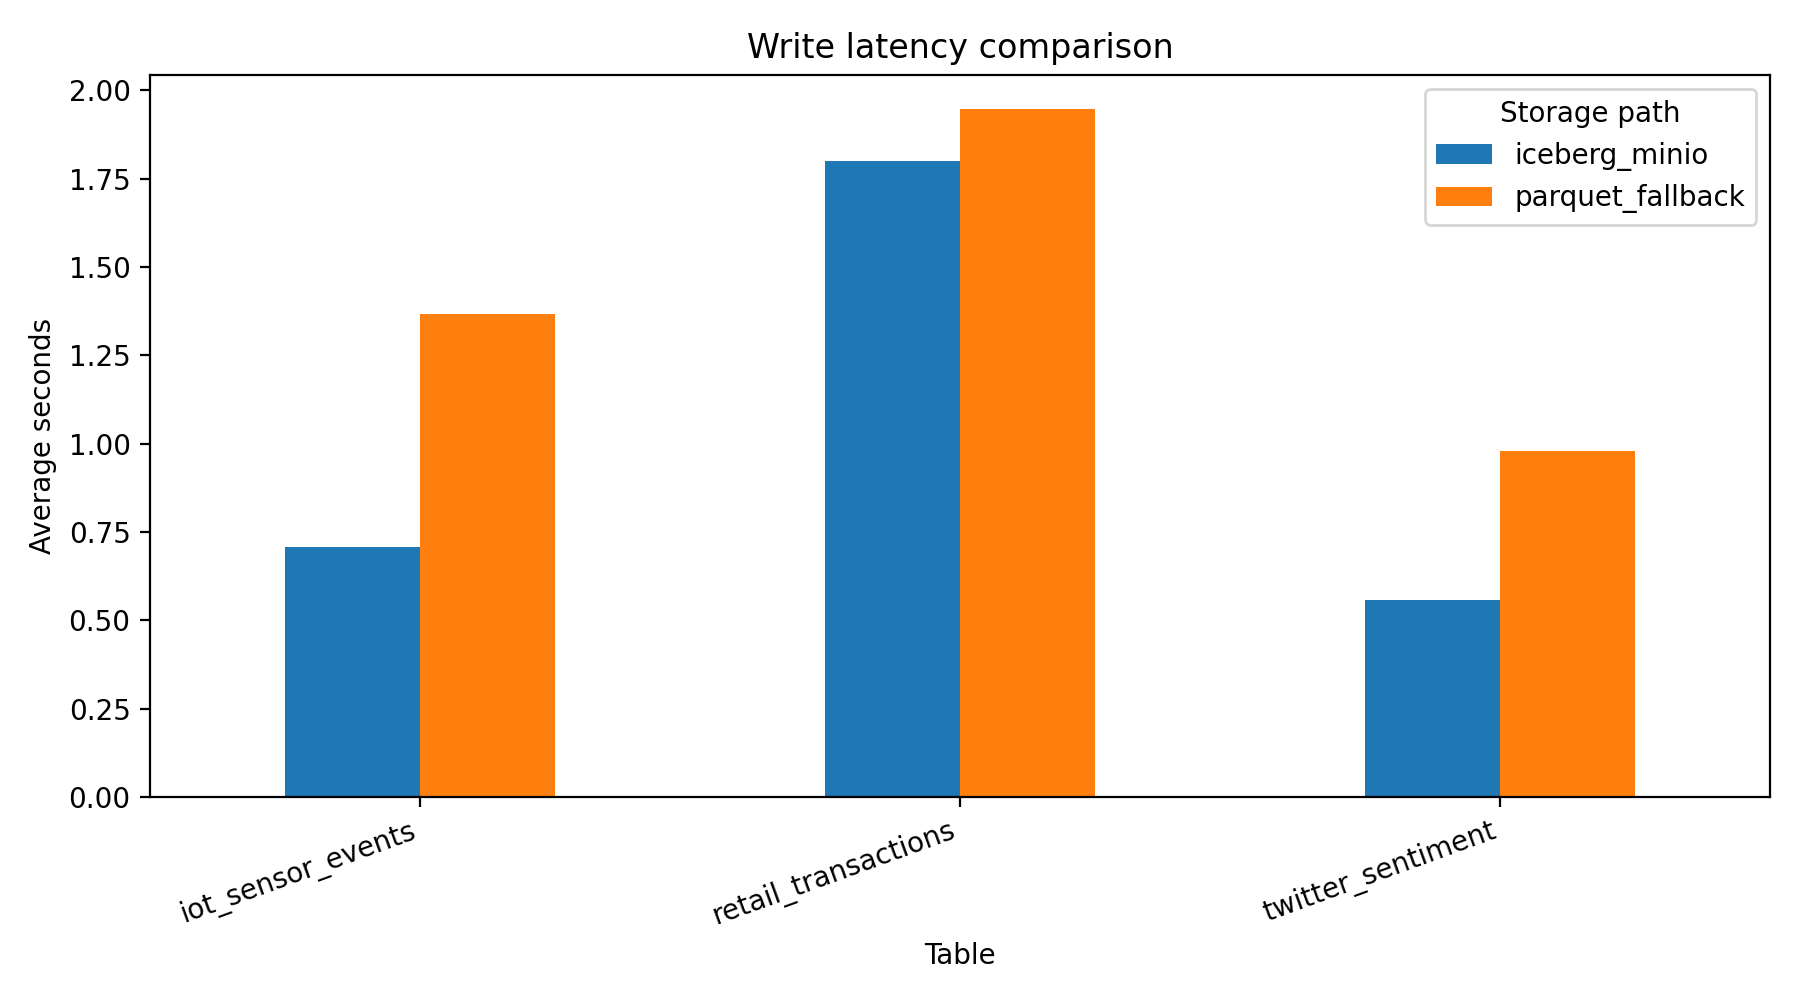
\includegraphics[width=0.48\textwidth]{write_latency_comparison.png}
\caption{So sánh thời gian ghi trung bình giữa Parquet fallback và Iceberg.}
\label{fig:write-latency}
\end{figure}

\begin{figure}[htbp]
\centering
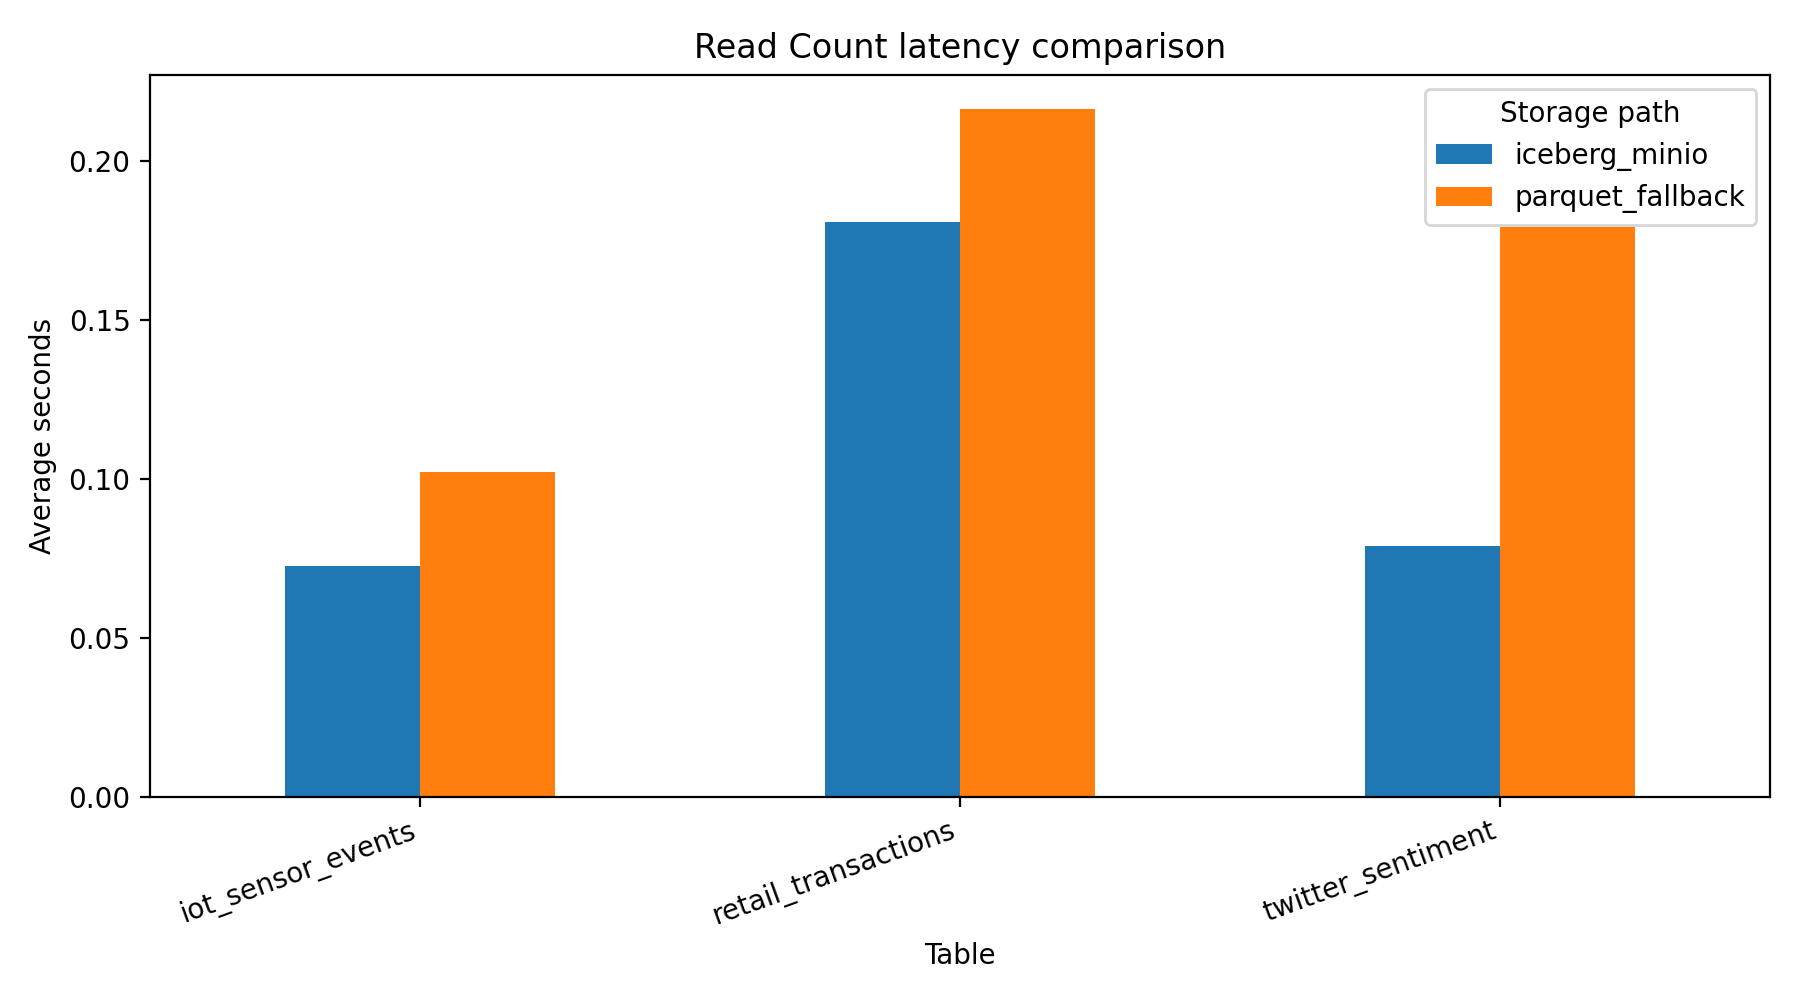
\includegraphics[width=0.48\textwidth]{read_latency_comparison.png}
\caption{So sánh thời gian đọc/đếm trung bình giữa Parquet fallback và Iceberg.}
\label{fig:read-latency}
\end{figure}

\begin{figure}[htbp]
\centering
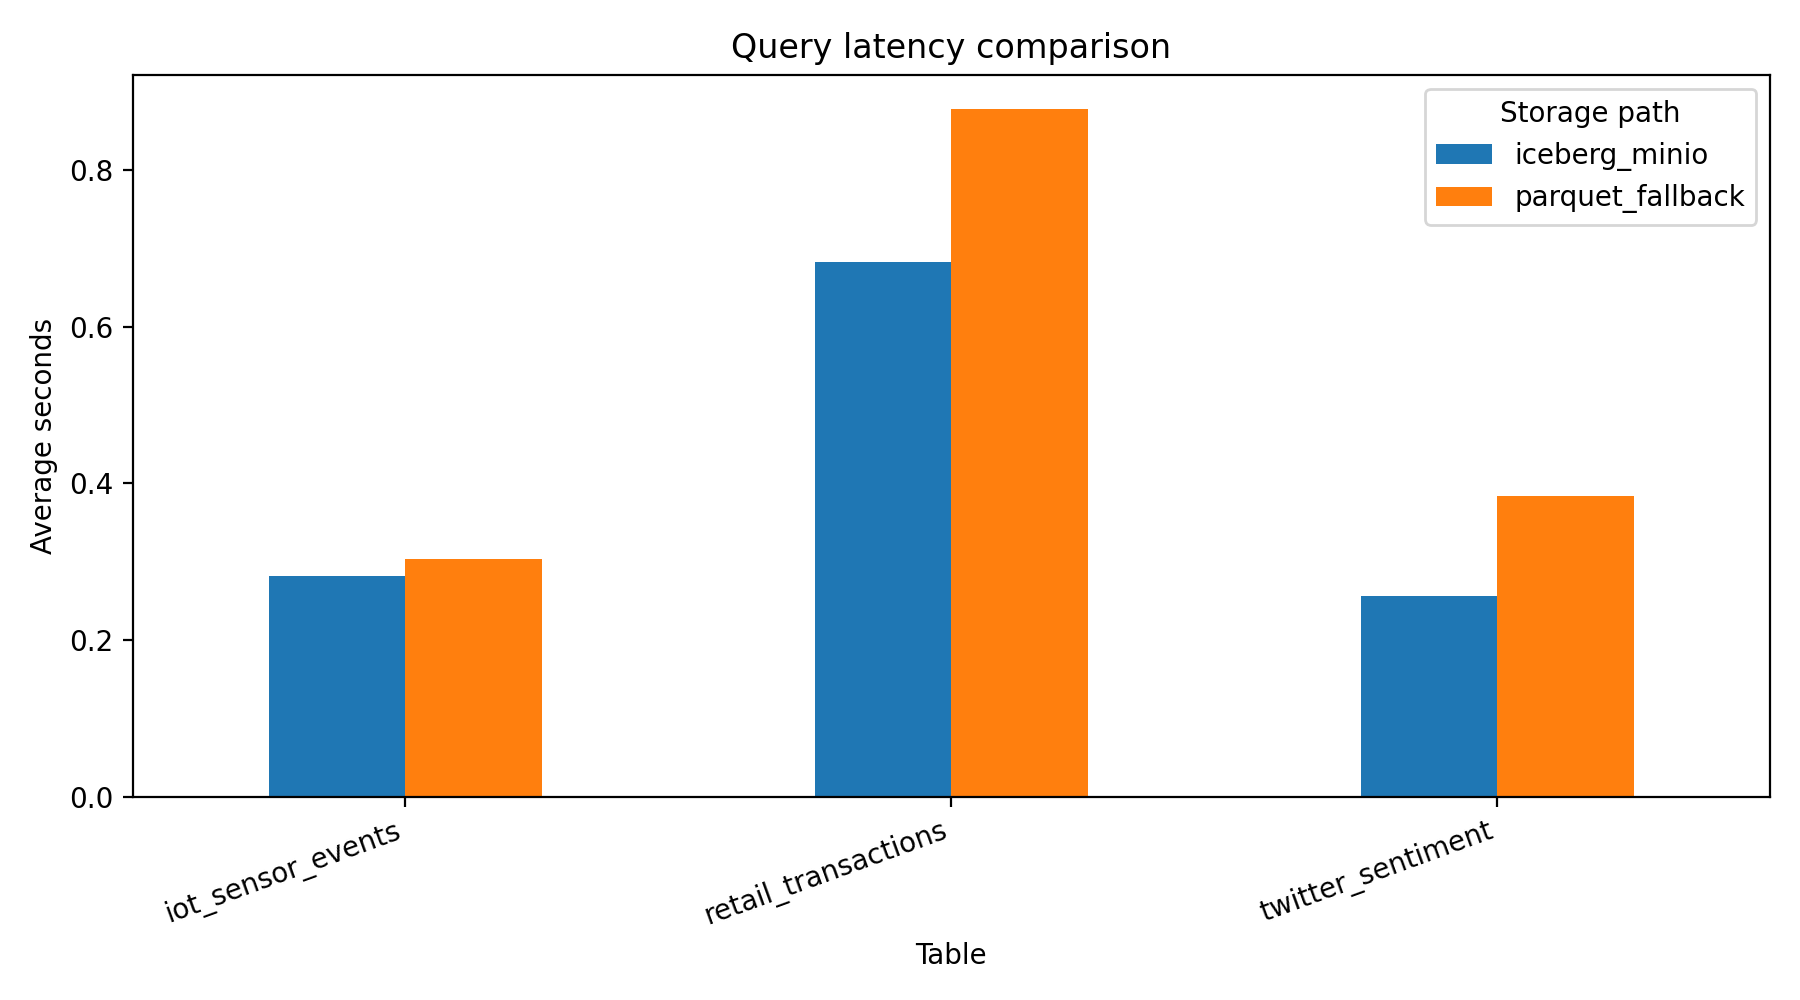
\includegraphics[width=0.48\textwidth]{query_latency_comparison.png}
\caption{So sánh thời gian truy vấn tổng hợp trung bình giữa Parquet fallback và Iceberg.}
\label{fig:query-latency}
\end{figure}

\subsection{Ghi chú về dữ liệu retail}

CSV retail ban đầu có 541.909 dòng sau bước chuẩn hóa bằng pandas. Trong benchmark Spark, các dòng không hợp lệ hoặc không đạt điều kiện làm sạch bị loại bỏ, bao gồm timestamp không hợp lệ, quantity không dương hoặc unit price âm. Vì vậy số dòng benchmark retail là 531.283. Việc ghi rõ khác biệt này giúp tránh nhầm lẫn giữa số dòng raw/chuẩn hóa ban đầu và số dòng thật sự đi qua workload đo thời gian.

\section{Đối chiếu với nghiên cứu và nguồn công khai}

Bảng~\ref{tab:public-validation} đối chiếu các nhận định từ nguồn học thuật/chính thức với quan sát trong prototype UniLake. Mục tiêu của bảng là phân biệt rõ điều gì đã được benchmark local hỗ trợ, điều gì chỉ được hỗ trợ ở mức kiến trúc, và điều gì chưa được kiểm chứng.

\begin{table*}[htbp]
\centering
\caption{Đối chiếu nguồn công khai với quan sát cục bộ}
\label{tab:public-validation}
\begin{tabularx}{\textwidth}{X p{0.18\textwidth} X p{0.16\textwidth} X}
\toprule
Nhận định công khai & Loại nguồn & Quan sát trong UniLake & Mức độ hỗ trợ & Diễn giải \\
\midrule
Lakehouse thống nhất data lake và data warehouse bằng định dạng mở, metadata và khả năng hỗ trợ analytics/ML. & Bài báo học thuật~\cite{lakehousePaper} & UniLake dùng MinIO, Parquet và Iceberg metadata trong một workflow Spark. & Hỗ trợ một phần & Đúng ở mức prototype kiến trúc, chưa chứng minh production-scale. \\
Spark là engine thống nhất cho batch, SQL, streaming và ML. & Bài báo/tài liệu~\cite{sparkCacm,sparkParquetDocs} & Benchmark dùng Spark cho cả làm sạch, ghi, đọc và Spark SQL. & Hỗ trợ trực tiếp & Engine xử lý được giữ cố định để so sánh storage/table layer. \\
Parquet là định dạng file cột phù hợp workload phân tích. & Tài liệu Spark và nền tảng Dremel~\cite{sparkParquetDocs,dremelPaper} & Parquet fallback ghi/đọc thành công trên cả ba bảng. & Hỗ trợ trực tiếp & Parquet là baseline hợp lệ cho data lake file-based. \\
Iceberg quản lý bảng qua metadata, snapshot và manifest; có thể quản lý file Parquet/Avro/ORC. & Đặc tả chính thức~\cite{icebergSpec} & Iceberg table được tạo trong warehouse MinIO bằng Spark. & Hỗ trợ kiến trúc & Prototype xác nhận workflow table format, không biến Iceberg thành file format thay thế Parquet. \\
Iceberg Spark hỗ trợ DataFrameWriterV2. & Tài liệu chính thức~\cite{icebergSparkWrites} & Script dùng \texttt{writeTo(...).using("iceberg").create()}. & Hỗ trợ trực tiếp & 18/18 dòng benchmark có \texttt{status=OK}. \\
Trino/StarRocks có thể truy vấn Iceberg qua connector/catalog. & Tài liệu chính thức~\cite{trinoIcebergDocs,starrocksIcebergDocs} & Trino/StarRocks chưa được chạy trong benchmark. & Chưa kiểm chứng & Phù hợp future work, không dùng làm bằng chứng hiệu năng hiện tại. \\
Iceberg nhanh hơn Parquet trong mọi workload. & Không có bằng chứng tổng quát trong phạm vi khảo sát & Benchmark local ghi nhận Iceberg thấp hơn Parquet fallback trong lần chạy này. & Chỉ hỗ trợ cục bộ và có điều kiện & Không khái quát hóa; cần workload, file layout và cụm lớn hơn để kết luận rộng. \\
\bottomrule
\end{tabularx}
\end{table*}

Kết quả đối chiếu cho thấy UniLake hỗ trợ tốt các nhận định về workflow và kiến trúc lakehouse, nhưng chỉ cung cấp bằng chứng hiệu năng ở phạm vi local. Đây là điểm quan trọng khi viết kết luận: lợi ích cốt lõi của Iceberg trong báo cáo nên được trình bày là quản lý bảng, metadata, snapshot và khả năng mở rộng engine, còn lợi thế thời gian chạy chỉ là quan sát cục bộ trong lần benchmark này.

\section{Thảo luận}

\subsection{Ý nghĩa của kết quả local}

Benchmark cho thấy đường Iceberg có thời gian trung bình thấp hơn Parquet fallback trong các thao tác được đo. Tuy nhiên, cần đọc kết quả này cùng với độ lệch chuẩn. Ví dụ, \texttt{retail\_transactions} có độ lệch chuẩn lớn ở thao tác ghi và truy vấn, đặc biệt do lần chạy đầu thường chịu ảnh hưởng của warm-up, cache, planning hoặc trạng thái container. Vì vậy, thay vì nhấn mạnh một kết luận tuyệt đối về tốc độ, báo cáo xem kết quả này như bằng chứng rằng workflow Iceberg trên MinIO có thể chạy thành công và có hiệu năng local cạnh tranh với Parquet fallback.

\subsection{Vì sao không so sánh legacy production đầy đủ?}

Một benchmark hoàn toàn đối xứng giữa legacy và modern stack sẽ cần dựng Kafka, HDFS, Spark cluster, Trino/Presto, object storage, catalog và các query workload tương đương. Nếu chỉ dựng một phần hoặc cấu hình không cân bằng, kết quả có thể phản ánh tài nguyên Docker hơn là khác biệt kiến trúc. Vì vậy UniLake chọn cách tách biệt: legacy stack được phân tích qua bài báo và tài liệu kiến trúc; benchmark local chỉ so sánh Parquet fallback và Iceberg bằng cùng Spark engine.

\subsection{Vai trò của Parquet trong lakehouse}

Một hiểu nhầm phổ biến là Iceberg thay thế Parquet. Trong thực tế, Iceberg quản lý bảng còn Parquet thường vẫn là định dạng file vật lý. Vì vậy, kết luận đúng không phải ``Iceberg tốt hơn Parquet'', mà là ``trên cùng một file format cột, table format như Iceberg bổ sung metadata, snapshot và quản lý schema/partition''. Benchmark UniLake được thiết kế để tránh lỗi diễn giải này.

\subsection{Hạn chế}

Các hạn chế chính gồm: benchmark chạy trên một máy cục bộ, số lần chạy là 3, dữ liệu vẫn nhỏ so với production, Spark chạy local mode, MinIO chạy trong Docker, và chưa có concurrent readers/writers. Báo cáo cũng chưa kiểm thử schema evolution, time travel, partition evolution, compaction hoặc engine interoperability bằng Trino/StarRocks. Những phần này cần được xem là hướng mở rộng nếu UniLake được phát triển thành benchmark sâu hơn.

\section{Khuyến nghị và kết luận}

\subsection{Khuyến nghị}

Đối với phạm vi học tập và prototype, UniLake nên giữ thiết kế Docker-first với Spark, MinIO và Iceberg làm lõi. Parquet fallback vẫn cần được duy trì vì nó là baseline đơn giản, dễ debug và giúp pipeline tiếp tục chạy nếu Iceberg/S3A gặp lỗi. Iceberg nên được dùng để minh họa lợi ích table format: metadata, snapshot, schema evolution và khả năng tích hợp nhiều engine.

Đối với hướng mở rộng, nhóm nên bổ sung bốn nhóm thí nghiệm. Thứ nhất là schema evolution, ví dụ thêm cột mới vào bảng sentiment hoặc IoT và kiểm tra khả năng đọc dữ liệu cũ. Thứ hai là snapshot/time travel để chứng minh rõ lợi ích table-management của Iceberg. Thứ ba là compaction/file layout, vì file nhỏ có thể ảnh hưởng đáng kể đến hiệu năng local. Thứ tư là thêm Trino hoặc StarRocks để kiểm chứng multi-engine analytics thay vì chỉ dùng Spark SQL.

\subsection{Kết luận}

Báo cáo đã trình bày UniLake như một nguyên mẫu so sánh giữa đường Spark + Parquet fallback và Spark + Iceberg table trên MinIO, đồng thời đặt thực nghiệm này trong bối cảnh legacy Big Data stack và modern lakehouse architecture. Kết quả benchmark local trên ba bảng thực tế cho thấy Iceberg có thời gian trung bình thấp hơn Parquet fallback trong lần chạy hiện tại. Tuy nhiên, kết quả này chỉ là bằng chứng cục bộ và không chứng minh Iceberg luôn nhanh hơn Parquet.

Đóng góp chính của UniLake nằm ở quy trình thực nghiệm có thể tái lập, cách tách biệt bằng chứng local với nguồn học thuật/công khai, và cách diễn giải đúng quan hệ giữa file format và table format. Trong phạm vi đề tài, modern lakehouse stack không thay thế tuyệt đối legacy stack; nó phù hợp hơn với mục tiêu quản lý bảng, metadata, snapshot và tái lập local, trong khi legacy stack vẫn có lợi thế về độ trưởng thành và hệ sinh thái production.


\bibliographystyle{IEEEtran}
\bibliography{references}

\end{document}
